\begin{remark*}[Exposition]
Before metric topology begins, the metric already supplies quantitative
measurements.  It measures the distance between two points, the spread of a
set, the distance from a point to a set, and the separation between two sets.
These distance notions are the numerical layer beneath balls, neighborhoods,
closedness, limit points, and convergence.
\end{remark*}

\begin{definitionbox}{Definition --- Diameter}
\begin{definition}[Diameter]\label{def:metric-diameter}
Let \((X,d)\) be a metric space and let \(A\subseteq X\) be nonempty.  The
\emph{diameter} of \(A\) is
\[
  \operatorname{diam}(A)
  :=
  \sup\{\,d(a,b):a,b\in A\,\},
\]
whenever this supremum is finite, and is \(+\infty\) otherwise.
\end{definition}
\end{definitionbox}

\begin{remark*}[Standard quantified statement]
\[
\operatorname{diam}(A)
=
\sup\{\,d(a,b):a,b\in A\,\}.
\]
\end{remark*}

\begin{remark*}[Interpretation]
The diameter records the largest distance needed to travel between two points
of \(A\).  It measures internal spread rather than location.
\end{remark*}

\begin{dependencies}
\begin{itemize}
  \item \hyperref[def:metric-space]{Definition: Metric Space}
\end{itemize}
\end{dependencies}

\begin{definitionbox}{Definition --- Distance from a Point to a Set}
\begin{definition}[Distance from a Point to a Set]\label{def:metric-point-set-distance}
Let \((X,d)\) be a metric space, let \(x\in X\), and let
\(A\subseteq X\) be nonempty.  The \emph{distance from \(x\) to \(A\)} is
\[
  d(x,A):=\inf\{\,d(x,a):a\in A\,\}.
\]
\end{definition}
\end{definitionbox}

\begin{remark*}[Standard quantified statement]
\[
d(x,A)=\inf_{a\in A}d(x,a).
\]
\end{remark*}

\begin{remark*}[Interpretation]
The number \(d(x,A)\) measures how close \(x\) can get to \(A\).  The
infimum may be achieved by a point of \(A\), but it need not be achieved in
every metric space.
\end{remark*}

\begin{dependencies}
\begin{itemize}
  \item \hyperref[def:metric-space]{Definition: Metric Space}
\end{itemize}
\end{dependencies}

\begin{definitionbox}{Definition --- Distance Between Sets}
\begin{definition}[Distance Between Sets]\label{def:metric-set-distance}
Let \((X,d)\) be a metric space, and let \(A,B\subseteq X\) be nonempty.  The
\emph{distance between \(A\) and \(B\)} is
\[
  d(A,B):=\inf\{\,d(a,b):a\in A,\ b\in B\,\}.
\]
\end{definition}
\end{definitionbox}

\begin{remark*}[Standard quantified statement]
\[
d(A,B)=\inf_{a\in A,\ b\in B}d(a,b).
\]
\end{remark*}

\begin{remark*}[Interpretation]
Set distance records the smallest separation that points of the two sets can
approach.  Distinct sets can have distance \(0\) if they touch in the limit.
\end{remark*}

\begin{dependencies}
\begin{itemize}
  \item \hyperref[def:metric-space]{Definition: Metric Space}
\end{itemize}
\end{dependencies}

\begin{theorembox}{Theorem}
\begin{theorem}[Distance to a Union]\label{thm:metric-distance-to-union}
Let \((X,d)\) be a metric space, let \(x\in X\), and let \(A,B\subseteq X\)
be nonempty.  Then
\[
  d(x,A\cup B)=\min\{d(x,A),d(x,B)\}.
\]

\smallskip
\noindent
\hyperref[prf:metric-distance-to-union]{\textit{Go to proof.}}
\end{theorem}
\end{theorembox}

\begin{remark*}[Standard quantified statement]
\[
d(x,A\cup B)=\min\{d(x,A),d(x,B)\}.
\]
\end{remark*}

\begin{remark*}[Interpretation]
To get close to a union, it is enough to get close to one of its pieces.  The
nearest piece determines the distance.
\end{remark*}

\begin{dependencies}
\begin{itemize}
  \item \hyperref[def:metric-point-set-distance]{Definition: Distance from a Point to a Set}
\end{itemize}
\end{dependencies}

\begin{theorembox}{Theorem}
\begin{theorem}[Distance to an Intersection Bound]
\label{thm:metric-distance-to-intersection-bound}
Let \((X,d)\) be a metric space, let \(x\in X\), and let
\(A,B\subseteq X\) have nonempty intersection.  Then
\[
  d(x,A\cap B)\geq \max\{d(x,A),d(x,B)\}.
\]

\smallskip
\noindent
\hyperref[prf:metric-distance-to-intersection-bound]{\textit{Go to proof.}}
\end{theorem}
\end{theorembox}

\begin{remark*}[Standard quantified statement]
\[
A\cap B\neq\varnothing
\Longrightarrow
d(x,A\cap B)\geq \max\{d(x,A),d(x,B)\}.
\]
\end{remark*}

\begin{remark*}[Interpretation]
An intersection has fewer candidate points than either set alone.  Fewer
points can only make the infimum distance larger, not smaller.
\end{remark*}

\begin{dependencies}
\begin{itemize}
  \item \hyperref[def:metric-point-set-distance]{Definition: Distance from a Point to a Set}
\end{itemize}
\end{dependencies}

\begin{definitionbox}{Definition --- Metric Bounded Set}
\begin{definition}[Metric Bounded Set]\label{def:metric-bounded-set}
Let \((X,d)\) be a metric space and let \(A\subseteq X\).  The set \(A\) is
\emph{bounded} if there exist \(x\in X\) and \(R>0\) such that
\[
  d(x,a)\leq R
\]
for every \(a\in A\).
\end{definition}
\end{definitionbox}

\begin{remark*}[Standard quantified statement]
\[
A\text{ is bounded}
\quad\Longleftrightarrow\quad
\exists x\in X\,\exists R>0\,\forall a\in A{:}\ d(x,a)\leq R.
\]
\end{remark*}

\begin{remark*}[Interpretation]
A bounded set has finite spread from at least one center.  The center is
auxiliary: boundedness records finite reach, not a preferred location.
Important trap: an infinite set can be bounded; for example,
\((0,1)\subseteq\mathbb{R}\) is bounded in the usual metric.
\end{remark*}

\begin{remark*}[Examples]
In \(\mathbb{R}\) with the usual metric, the intervals \((0,1)\),
\([0,1]\), \((a,b)\), and \([a,b]\) are bounded whenever \(a<b\).  The rays
\((0,\infty)\) and \([0,\infty)\), and the whole line \(\mathbb{R}\), are not
bounded.
\end{remark*}

\begin{dependencies}
\begin{itemize}
  \item \hyperref[def:metric-space]{Definition: Metric Space}
\end{itemize}
\end{dependencies}

\begin{figure}[htbp]
\centering
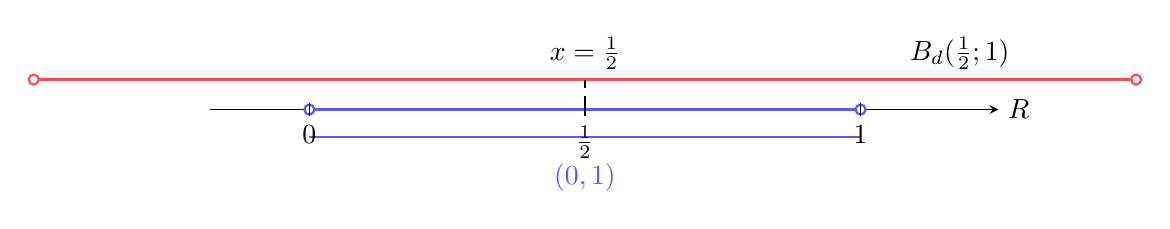
\begin{tikzpicture}[x=7cm,y=1cm,>=stealth]
  \draw[->] (-0.18,0) -- (1.25,0) node[right] {\(\mathbb{R}\)};

  \draw[very thick,blue!65] (0,0) -- (1,0);
  \draw[fill=white,draw=blue!65,thick] (0,0) circle (1.8pt);
  \draw[fill=white,draw=blue!65,thick] (1,0) circle (1.8pt);

  \draw[blue!65,thick] (0,-0.35) -- (1,-0.35)
    node[midway,below=6pt] {\((0,1)\)};

  \draw[red!70,thick] (-0.5,0.38) -- (1.5,0.38);
  \draw[fill=white,draw=red!70,thick] (-0.5,0.38) circle (1.8pt);
  \draw[fill=white,draw=red!70,thick] (1.5,0.38) circle (1.8pt);
  \draw[dashed] (0.5,0.38) -- (0.5,-0.08);
  \node[above] at (0.5,0.38) {\(x=\frac12\)};
  \node[above] at (1.18,0.38) {\(B_d(\frac12;1)\)};

  \foreach \p/\lab in {0/0,0.5/\frac12,1/1}
  {
    \draw (\p,0.08) -- (\p,-0.08);
    \node[below] at (\p,-0.08) {\(\lab\)};
  }
\end{tikzpicture}

\caption{In \(\mathbb{R}\), the interval \((0,1)\) is bounded because every
point of the interval is within distance \(1\) of \(1/2\).}
\label{fig:bounded-interval-r}
\end{figure}

\begin{figure}[htbp]
\centering
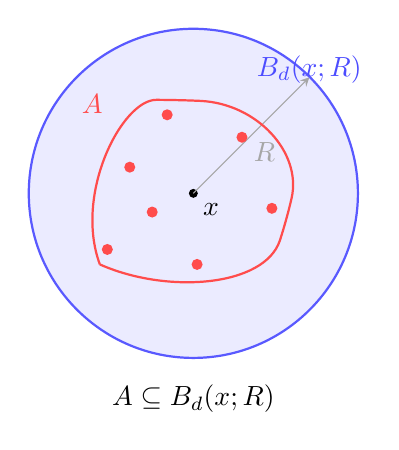
\begin{tikzpicture}[scale=0.95,>=stealth]
  \fill[blue!8] (0,0) circle (2.2);
  \draw[blue!65,thick] (0,0) circle (2.2);
  \node[blue!70] at (1.55,1.65) {\(B_d(x;R)\)};

  \fill[black] (0,0) circle (1.7pt);
  \node[below right] at (0,0) {\(x\)};
  \draw[->,gray!70] (0,0) -- (1.55,1.55);
  \node[gray!70] at (0.95,0.55) {\(R\)};

  \foreach \p in {(-0.85,0.35),(-0.35,1.05),(0.65,0.75),(1.05,-0.2),
                  (0.05,-0.95),(-1.15,-0.75),(-0.55,-0.25)}
  {
    \fill[red!70] \p circle (2.1pt);
  }

  \draw[red!70,thick,rounded corners=8pt]
    (-1.25,-0.95) .. controls (-1.6,0.0) and (-0.95,1.25) .. (-0.2,1.25)
    .. controls (0.85,1.2) and (1.45,0.55) .. (1.25,-0.35)
    .. controls (0.95,-1.25) and (-0.35,-1.35) .. (-1.25,-0.95);
  \node[red!70] at (-1.35,1.2) {\(A\)};

  \node at (0,-2.75) {\(A\subseteq B_d(x;R)\)};
\end{tikzpicture}

\caption{An arbitrary subset \(A\) of a metric space is bounded when all of
its points lie within one finite distance bound from a chosen center.}
\label{fig:bounded-arbitrary-set}
\end{figure}

\begin{theorembox}{Theorem}
\begin{theorem}[Equivalent Boundedness Criterion]
\label{thm:metric-equivalent-boundedness-criterion}
Let \((X,d)\) be a metric space and let \(A\subseteq X\).  Then \(A\) is
bounded if and only if there exist \(x\in X\) and \(R>0\) such that
\[
  d(x,a)<R
\]
for every \(a\in A\).
\end{theorem}
\end{theorembox}

\begin{remark*}[Standard quantified statement]
\[
A\text{ is bounded}
\quad\Longleftrightarrow\quad
\exists x\in X\,\exists R>0\,\forall a\in A{:}\ d(x,a)<R.
\]
\end{remark*}

\begin{remark*}[Interpretation]
Strict and non-strict radius bounds are equivalent after enlarging the radius.
Both express the same finite-spread condition.
\end{remark*}

\begin{dependencies}
\begin{itemize}
  \item \hyperref[def:metric-bounded-set]{Definition: Metric Bounded Set}
\end{itemize}
\end{dependencies}

\begin{theorembox}{Theorem}
\begin{theorem}[Center Independence]\label{thm:metric-bounded-center-independence}
Let \((X,d)\) be a metric space.  If \(A\subseteq X\) and there exist
\(x\in X\) and \(R>0\) such that \(d(x,a)\leq R\) for every \(a\in A\), then
for every \(y\in X\),
\[
  d(y,a)\leq R+d(x,y)
\]
for every \(a\in A\).  Thus boundedness does not depend on the chosen center.
\end{theorem}
\end{theorembox}

\begin{remark*}[Standard quantified statement]
\[
\bigl(\forall a\in A{:}\ d(x,a)\leq R\bigr)
\Longrightarrow
\forall y\in X\,\forall a\in A{:}\ d(y,a)\leq R+d(x,y).
\]
\end{remark*}

\begin{remark*}[Interpretation]
Changing centers costs at most the distance between the old center and the
new center.  The triangle inequality transports one finite bound to any other
center.
\end{remark*}

\begin{dependencies}
\begin{itemize}
  \item \hyperref[def:metric-bounded-set]{Definition: Metric Bounded Set}
\end{itemize}
\end{dependencies}

\begin{theorembox}{Theorem}
\begin{theorem}[Subsets of Bounded Sets Are Bounded]
\label{thm:metric-subsets-bounded-sets-bounded}
Let \((X,d)\) be a metric space.  If \(A\subseteq B\subseteq X\) and \(B\) is
bounded, then \(A\) is bounded.
\end{theorem}
\end{theorembox}

\begin{remark*}[Standard quantified statement]
\[
A\subseteq B\subseteq X
\;\land\;
B\text{ is bounded}
\Longrightarrow
A\text{ is bounded}.
\]
\end{remark*}

\begin{remark*}[Interpretation]
A subset cannot spread out more than the set containing it.  Any bound for
\(B\) automatically bounds \(A\).
\end{remark*}

\begin{dependencies}
\begin{itemize}
  \item \hyperref[def:metric-bounded-set]{Definition: Metric Bounded Set}
\end{itemize}
\end{dependencies}

\begin{theorembox}{Theorem}
\begin{theorem}[Finite Sets Are Bounded]\label{thm:metric-finite-sets-bounded}
Every finite subset of a metric space is bounded.
\end{theorem}
\end{theorembox}

\begin{remark*}[Standard quantified statement]
\[
A\subseteq X
\;\land\;
A\text{ is finite}
\Longrightarrow
A\text{ is bounded}.
\]
\end{remark*}

\begin{remark*}[Interpretation]
Only finitely many distances must be controlled.  Choosing one center and a
bound larger than all distances from that center captures the whole finite
set.
\end{remark*}

\begin{dependencies}
\begin{itemize}
  \item \hyperref[def:metric-bounded-set]{Definition: Metric Bounded Set}
\end{itemize}
\end{dependencies}

\begin{theorembox}{Theorem}
\begin{theorem}[Finite Unions of Bounded Sets Are Bounded]
\label{thm:metric-finite-unions-bounded-sets-bounded}
Let \((X,d)\) be a metric space, let \(n\in\mathbb{N}\), and let
\(A_1,\ldots,A_n\subseteq X\).  If \(A_1,\ldots,A_n\) are bounded, then
\[
  \bigcup_{k=1}^n A_k
\]
is bounded.
\end{theorem}
\end{theorembox}

\begin{remark*}[Standard quantified statement]
\[
\bigl(\forall k\in\{1,\ldots,n\}{:}\ A_k\text{ is bounded}\bigr)
\Longrightarrow
\bigcup_{k=1}^n A_k\text{ is bounded}.
\]
\end{remark*}

\begin{remark*}[Interpretation]
Each bounded set has finite spread.  A finite union still has only finitely
many centers and bounds to absorb into one sufficiently large bound.
\end{remark*}

\begin{dependencies}
\begin{itemize}
  \item \hyperref[def:metric-bounded-set]{Definition: Metric Bounded Set}
  \item \hyperref[thm:metric-bounded-center-independence]{Theorem: Center Independence}
\end{itemize}
\end{dependencies}

\begin{theorembox}{Theorem}
\begin{theorem}[Boundedness via Diameter]\label{thm:metric-boundedness-via-diameter}
Let \((X,d)\) be a metric space and let \(A\subseteq X\) be nonempty.  Then
\(A\) is bounded if and only if there exists \(C>0\) such that
\[
  d(a,b)\leq C
\]
for all \(a,b\in A\).
\end{theorem}
\end{theorembox}

\begin{remark*}[Standard quantified statement]
\[
A\neq\varnothing
\Longrightarrow
\Bigl(
A\text{ is bounded}
\Longleftrightarrow
\exists C>0\,\forall a,b\in A{:}\ d(a,b)\leq C
\Bigr).
\]
\end{remark*}

\begin{remark*}[Interpretation]
For nonempty sets, boundedness can be measured internally: all pairwise
distances must be uniformly bounded.  This is the diameter viewpoint.
\end{remark*}

\begin{dependencies}
\begin{itemize}
  \item \hyperref[def:metric-bounded-set]{Definition: Metric Bounded Set}
  \item \hyperref[def:metric-diameter]{Definition: Diameter}
\end{itemize}
\end{dependencies}

\begin{theorembox}{Theorem}
\begin{theorem}[Closure of a Bounded Set Is Bounded]
\label{thm:metric-closure-bounded-set-bounded}
Let \((X,d)\) be a metric space.  If \(A\subseteq X\) is bounded, then
\(\operatorname{cl}(A)\) is bounded.
\end{theorem}
\end{theorembox}

\begin{remark*}[Standard quantified statement]
\[
A\text{ is bounded}
\Longrightarrow
\operatorname{cl}(A)\text{ is bounded}.
\]
\end{remark*}

\begin{remark*}[Interpretation]
Passing to the closure may add limit points, but it does not create points
arbitrarily far away.  A slightly enlarged bound still captures the closure.
\end{remark*}

\begin{dependencies}
\begin{itemize}
  \item \hyperref[def:metric-bounded-set]{Definition: Metric Bounded Set}
  \item \hyperref[def:metric-closure]{Definition: Metric Closure}
\end{itemize}
\end{dependencies}

\begin{theorembox}{Theorem}
\begin{theorem}[Compact Sets Are Bounded]\label{thm:metric-compact-sets-bounded}
Every compact subset of a metric space is bounded.
\end{theorem}
\end{theorembox}

\begin{remark*}[Standard quantified statement]
\[
K\subseteq X
\;\land\;
K\text{ is compact}
\Longrightarrow
K\text{ is bounded}.
\]
\end{remark*}

\begin{remark*}[Interpretation]
The open balls centered at any fixed point cover the compact set as their
radii grow.  Compactness reduces this cover to finitely many radii, and the
largest one bounds the set.
\end{remark*}

\begin{dependencies}
\begin{itemize}
  \item \hyperref[def:metric-bounded-set]{Definition: Metric Bounded Set}
\end{itemize}
\end{dependencies}

\begin{theorembox}{Theorem}
\begin{theorem}[Totally Bounded Sets Are Bounded]
\label{thm:metric-totally-bounded-sets-bounded}
Every totally bounded subset of a metric space is bounded.
\end{theorem}
\end{theorembox}

\begin{remark*}[Standard quantified statement]
\[
A\subseteq X
\;\land\;
A\text{ is totally bounded}
\Longrightarrow
A\text{ is bounded}.
\]
\end{remark*}

\begin{remark*}[Interpretation]
A totally bounded set can be covered by finitely many balls of one fixed
radius.  A finite collection of bounded balls has finite overall spread, so
the set is bounded.
\end{remark*}

\begin{dependencies}
\begin{itemize}
  \item \hyperref[def:metric-bounded-set]{Definition: Metric Bounded Set}
  \item \hyperref[thm:metric-finite-unions-bounded-sets-bounded]{Theorem: Finite Unions of Bounded Sets Are Bounded}
\end{itemize}
\end{dependencies}
